\section{Statistical Properties of Control Charts}
\noindent\rule[\linienAbstand]{\linewidth}{\linienDickeDick}
Aim of process control using control charts: Keep the process under statistical control.
Or, if it is not at the beginning, to put it into statistical control by improving production conditions.

\subsection{Interpretation of Control Charts}
\noindent\rule[\linienAbstand]{\linewidth}{\linienDicke}

\paragraph{Western Electric Rules}
\begin{enumerate}
  \item Any single data point falls outside the limit defined by UCL and LCL (beyond the 3$\sigma$-limit).
  \item 2. Two out of three consecutive points fall beyond the limit defined by $\frac{2}{3}$ UCL and $\frac{2}{3}$ LCL on the same side of the centreline (beyond the 2$\sigma$-limit).
  \item Four out of five consecutive points fall beyond the limit defined by $\frac{1}{3}$UCL and $\frac{1}{3}$ LCL on the same side of the centreline (beyond the 2$\sigma$-limit).
  \item Nine consecutive points fall on the same side of the centreline (so-called run).
\end{enumerate}

\begin{table}[H]
  \setlength{\tabcolsep}{0.2em}
  \footnotesize
  \begin{tabular}{p{\linewidth / 2 - 0.5em}@{\hskip 1em}p{\linewidth / 2 - 0.5em}}
    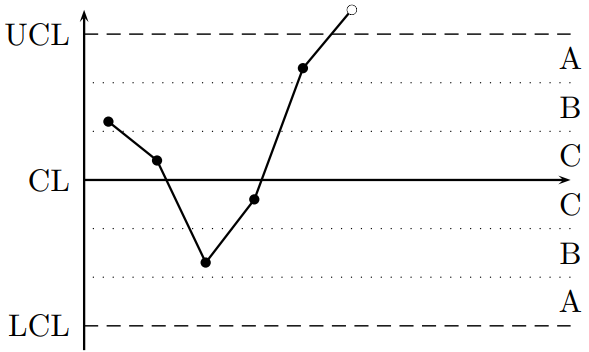
\includegraphics[width=\linewidth]{Pics/3.1.1.png}& 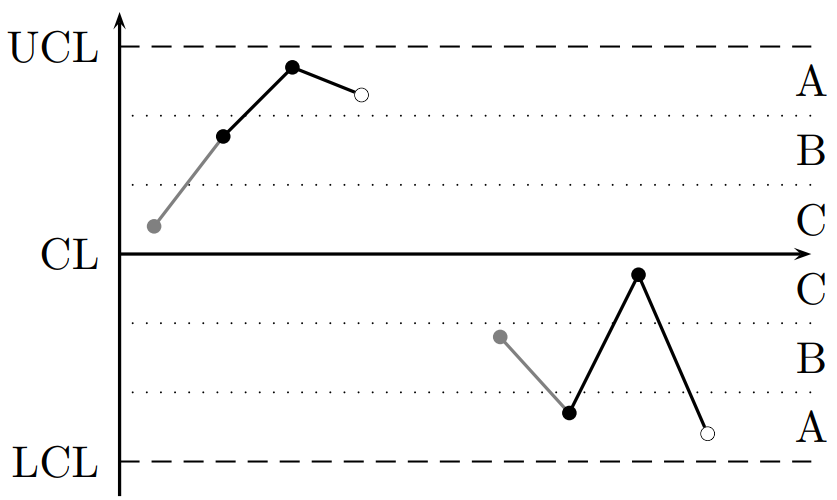
\includegraphics[width=\linewidth]{Pics/3.1.2.png} \\
    Rule 1: Any point beyond zone A. &
    Rule 2: Two out of three consecutive points fall on the same side in zone A or beyond.\\
    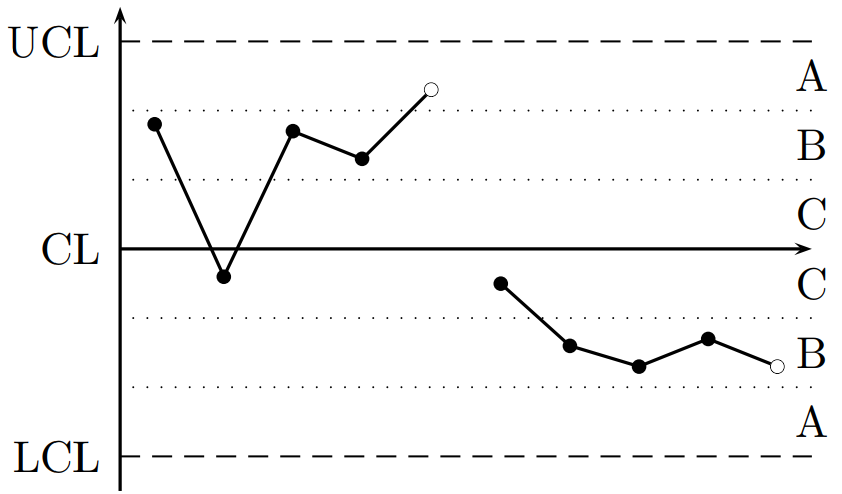
\includegraphics[width=\linewidth]{Pics/3.1.3.png}& 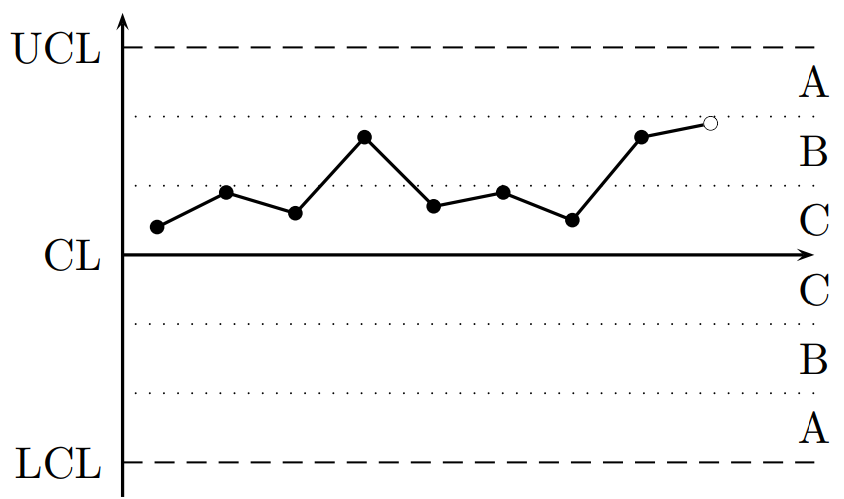
\includegraphics[width=\linewidth]{Pics/3.1.4.png} \\
    Rule 3: Four out of five consecutive points fall on the same side in zone B or beyond. &
    Rule 4: Nine consecutive points fall on the same side of the centreline.
  \end{tabular}
\end{table}

\subsection{Type I Error and Type II Error}
\noindent\rule[\linienAbstand]{\linewidth}{\linienDicke}
When monitoring a production process with a control chart, as with any statistical test, there are two wrong decisions possible.
\begin{equation}
  \begin{split}
    H_0:& \mu_0 = \mu \text{ i.e. process is not disturbed}\\
    H_1:& \mu_0 \neq \mu \text{ i.e. process is disturbed, } \mu_1 \text{ is true}
  \end{split}
\end{equation}
Denoted by:\\
 - $\mu_0$ the target value of the process\\
 - $\mu$ the considered statistic, eg. $\mu = \bar{x}$ or $\mu = R$\\
 - $\mu_1$ the true value of the considered statistic.\\

\textbf{Two wrong decisions possible:}\\
 - If a true null hypothesis $H_0$ is rejected we make a type I error. An intervention in the process is necessary, because the control limits are exceeded, although the process is not disturbed. This is called a false alarm.\\
 - If a false null hypothesis $H_0$ is accepted we make a type II error. There is no intervention, since the control limits are not exceeded, although the process is disturbed. This is called an omitted alarm\\

\textbf{Type I Error}\\
\begin{table}[H]
  \setlength{\tabcolsep}{0.2em}
  \footnotesize
  \begin{tabular}{p{\linewidth / 2 - 0.5em}@{\hskip 1em}p{\linewidth / 2 - 0.5em}}
    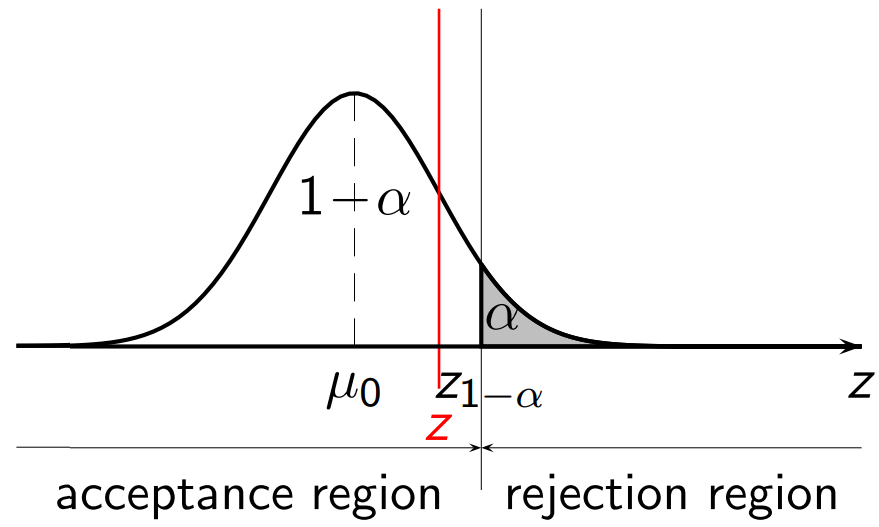
\includegraphics[width=\linewidth]{Pics/3.2.1.png}& 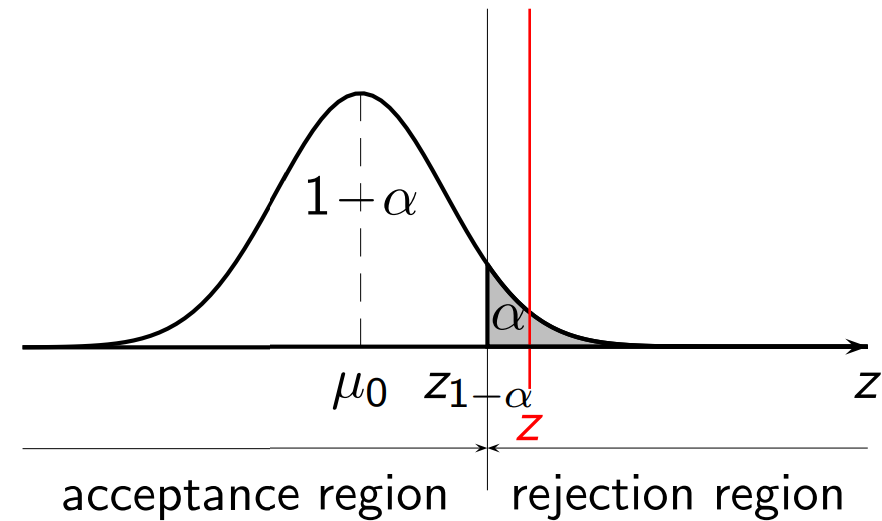
\includegraphics[width=\linewidth]{Pics/3.2.2.png} \\
    Let $h_0$ be true: Since $z < z_{1-\alpha}$ the null hypothesis is accepted. This is the right decision, which is made with probability $1-\alpha$. &
    Let $h_0$ be true: Since $z \geq z_{1-\alpha}$ the null hypothesis is rejected. This is the wrong decision (type I error), which is made with probability $\alpha$.
  \end{tabular}
\end{table}

\textbf{Type II Error}\\
\begin{table}[H]
  \setlength{\tabcolsep}{0.0em}
  \footnotesize
  \begin{tabular}{p{\linewidth / 2 - 0.5em}@{\hskip 1em}p{\linewidth / 2 - 0.5em}}
    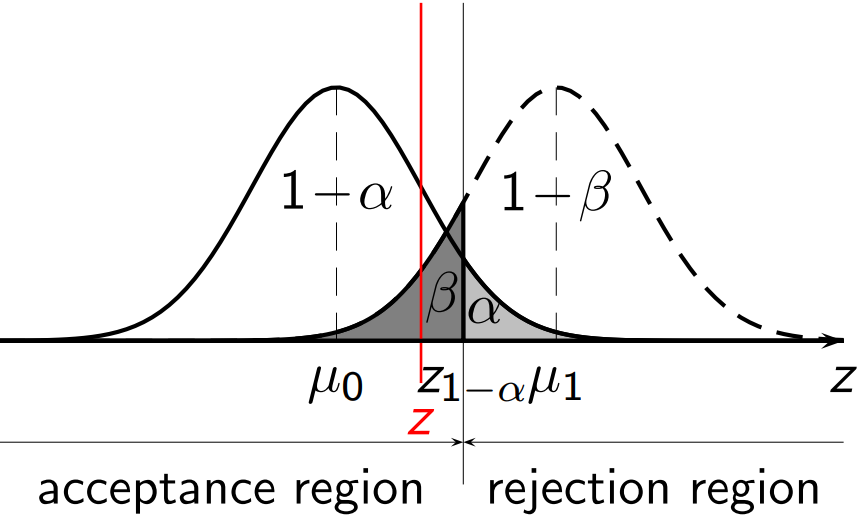
\includegraphics[width=\linewidth]{Pics/3.2.3.png}& 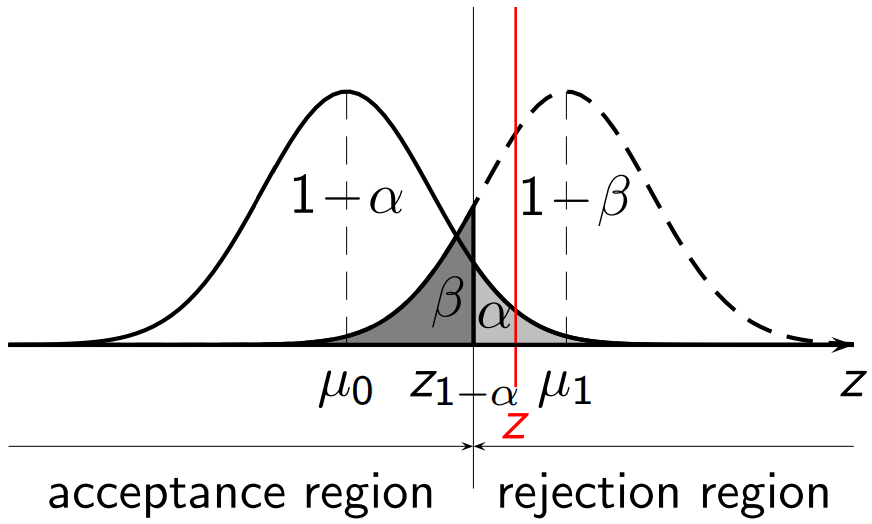
\includegraphics[width=\linewidth]{Pics/3.2.4.png} \\
    Let $H_0$ be false, $H_1$ true, i.e. the dashed density is true: Since $z < z_1-\alpha$ the null hypothesis is accepted. This is the wrong decision (type II error), which is made with probability $\beta$. &
    Let $H_0$ be false, $H_1$ true, i.e. the dashed density is true: Since $z \leq z_1-\alpha$ the null hypothesis is rejected. This is the correct decision, which is made with probability $1 - \beta$ (power).
  \end{tabular}
\end{table}

\subsection{Power Function and Operating Characteristic}
\noindent\rule[\linienAbstand]{\linewidth}{\linienDicke}
The power of a hypothesis test is the probability $1-\beta$ that the test correctly rejects the null hypothesis when the alternative hypothesis is true, i.e.
\begin{equation}
  \text{power} = P(\text{reject } H_0 | H_1 \text{ is true}) = 1-\beta
\end{equation}

\textbf{Power function}\\
Probability to reject the null hypothesis $H_0$ if $\mu_1$ is true.\\
\begin{equation}
  \delta = \frac{\mu_1 - \mu_0}{\sigma},
\end{equation}
or $\mu_1 = \delta\sigma + \mu_0$.\\
The variable $\delta$ is a normalized measure for the deviation of the disturbed from the undisturbed process in units of $\sigma$.\\
In statistical process control the power function is denoted by
\begin{equation}
  g(\mu_1) = g(\delta\sigma + \mu_0) = \tilde{g} (\delta).
\end{equation}
It is a measure for the probability of an intervention in the process.\\

 \textbf{Undisturbed Process}\\
 For an undisturbed process, i.e. $\mu = \mu_0$, we have
 \begin{equation}
   g(\mu_1) = \tilde{g} (0) = \alpha.
   \label{eq:3.3.a}
 \end{equation}

\textbf{Disturbed Process}\\
For a disturbed process we have
\begin{equation}
  \tilde{g}(\delta) = \Phi(\delta\sqrt{n} - z_q, 0, 1) + \Phi(-\delta\sqrt{n} - z_q, 0, 1)
  \label{eq:3.3.d}
\end{equation}
with $\Phi$ being
\begin{equation}
  \Phi(x, \mu, \sigma^2) = \frac{1}{\sqrt{2\pi\sigma^2}}\int^x_{-\infty}e^{-\frac{{(z-\mu)}^2}{2\sigma^2}}dz
\end{equation}


\subsection{Average Run Length}
\noindent\rule[\linienAbstand]{\linewidth}{\linienDicke}
If the $i_{RL}$-th sample is the first to result in an intervention, i.e. this sample is beyond the control limits, then $i_{RL}$ is called the run length of the control chart.\\
The ARL is the expected value of the probability i.e. the likelihood of exceeding the control limits when performing a test.
\begin{equation}
  ARL(\delta) = \frac{1}{p(\mu)} = \frac{1}{g(\mu_1)} = \frac{1}{\tilde{g}(\delta)}
\end{equation}

\textbf{Undisturbed Process}\\
If we have an undisturbed process with $\mu_1 = \mu_0$, i.e. with $\delta = 0$, then it follows from equation \ref{eq:3.3.a} that
\begin{equation}
  ARL(0) = \frac{1}{\alpha}.
\end{equation}

\textbf{Disturbed Process}\\
To determine the average run length of a disturbed process with $\mu = \mu_1$, i.e. $\sigma = \frac{\mu_1 - \mu_0}{\sigma}$ we use the power function $\tilde{g}(\delta)$ from equation \ref{eq:3.3.d}.

\subsection{Process Capability}
\noindent\rule[\linienAbstand]{\linewidth}{\linienDicke}
The specification limit (SL) is defined by
\begin{equation}
  SL = \frac{USL + LSL}{2}
\end{equation}

This performance is measured with so-called capability process ratios (PCR). The simplest process capability index is
\begin{equation}
  C_p = \frac{USL - LSL}{6\sigma}
\end{equation}
The capability process ratio $C_p$ expresses the ratio of the width of the tolerance range to the width of the process range.

\begin{itemize}
  \item $C_p = 1$ implies a reject rate of $\alpha \cdot 100\% = 0.27\%$.
  \item $C_p < 1$ implies a reject rate of more than $\alpha \cdot 100\% = 0.27\%$, i.e. the process capability is not guaranteed.
  \item $C_p > 1$ implies a reject rate of less than $\alpha \cdot 100\% = 0.27\%$,i.e. the process capability is guaranteed.

\end{itemize}
